% Restatement environment for results proved in the appendix
\newenvironment{restated}[1]{\par\smallskip\noindent\textbf{#1 (restated).}\ \itshape}{\par\smallskip}
\newcommand{\idea}{\par\noindent\textbf{Idea.}\ }
\newcommand{\step}[1]{\par\noindent\emph{Step #1.}\ }

\section{Overview of the Formal Results}\label[appendix]{app:summary}

\Cref{tab:results} lists every formal result, where it is stated, and what it assumes. Each proof in \cref{app:proofs} first restates the result, then gives the idea in a few sentences, and then proceeds in short numbered steps. \Cref{tab:notation} collects the notation.

\begin{table}[h]
\centering\scriptsize
\setlength{\tabcolsep}{4pt}
\begin{tabular}{@{}p{0.27\linewidth}p{0.45\linewidth}p{0.2\linewidth}@{}}
\toprule
Result & Statement in one line & Key assumptions \\
\midrule
\Cref{obs:first} (first-contact initialization) & Error-driven, episode-reset adapters predict with the frozen model at the first contact. & No feedback before commitment \\
\Cref{thm:confidence} (memory error) & Memory error $\le$ noise $+$ prior mismatch $+$ contamination; contamination is bounded by the filter's log loss. & \Cref{ass:main}; predictive weights \\
\Cref{rem:bias} (filtered weights) & Posterior-weighted updates converge to a biased value with shrinking intervals. & Fixed scoring models \\
\Cref{prop:first} (first-contact separation) & Cumulative first-contact bias $\le\sum\epsilon_e+\Delta_{\max}\times$ episode log loss; reset methods pay $\ge N_{\mathrm{shift}}\Delta_{\min}$. & Closed library \\
\Cref{cor:novel} (novel branch) & Extends \cref{prop:first} to a mixture that includes the new-context hypothesis. & Bound on novel-branch error \\
\Cref{cor:entropy} (entropy reference) & A KT predictor has log loss $\le N\widehat H(C\mid Y)+O(K|\mathcal Y|\log N)$. & Revealed labels \\
\Cref{lem:simulation}, \cref{cor:decision} (decision gap) & Prediction error along candidate rollouts bounds the committed-action gap. & Lipschitz dynamics, costs \\
\Cref{prop:composition} (composition) & Additive transfer to an unseen pair iff the observed-combination graph connects it; interactions leave a variance floor. & Exact stored means \\
\Cref{prop:voi} (value of information) & $\VOI\ge0$, and $\VOI=0$ when one action is optimal for all plausible states. & Fixed state and action set \\
\Cref{prop:safety} (latent safety) & Violations $\le\delta_sT+K_T(\bar S+2\gamma)/\gamma$ for any context and cue sequence. & Bounded scores, exact filter \\
\Cref{prop:recognition} (recognition time) & Expected steps to recognition $=(\ell_\star-\ell_0+\E[O_T])/D$. & i.i.d.\ increments \\
\bottomrule
\end{tabular}
\caption{Formal results and their assumptions.}
\label{tab:results}
\end{table}

\begin{table}[h]
\centering\scriptsize
\setlength{\tabcolsep}{4pt}
\begin{tabular}{@{}ll@{\hspace{14pt}}ll@{}}
\toprule
Symbol & Meaning & Symbol & Meaning \\
\midrule
$z_t,\,a_t$ & latent state, action & $f$ & frozen predictor \\
$c_e,\ c_t$ & true context (episode, step) & $\mu_c$ & mean residual of context $c$ \\
$U,\ \phi$ & correction subspace, features & $v_t=U^\top r_t$ & projected residual \\
$w_{c,i}$, $\widehat w_{c,i,t}$ & true / estimated weights (row $i$) & $m_c$ & latent correction of memory $c$ \\
$q_t(c)$ & belief \emph{before} observing $v_t$ & $\pi_t^+(c)$ & belief \emph{after} observing $v_t$ \\
$\pi_e(c)$ & pre-contact belief in episode $e$ & $y_e$ & visual cue \\
$\omega_{c,i,t}$ & update weight $q_t(c)/\sigma_i^2$ & $V_{c,i,t}$ & weighted design matrix \\
$P_{c,i},\ \nu_{c,i,t}$ & prior precision, prior mean & $\Delta_{\max}$ & largest residual difference \\
$h,\ L_h$ & latent safety function, Lipschitz constant & $b_{c,t}$ & safety margin of memory $c$ \\
$s_{c,t}$ & calibration score of memory $c$ & $\delta_s,\ \gamma$ & target miss rate, step size \\
\bottomrule
\end{tabular}
\caption{Notation used in the proofs. We write $\|x\|_A=\sqrt{x^\top Ax}$, and $\mathcal F_{t-1}$ for the history up to and including $(z_t,a_t)$, the cue and the true context $c_t$.}
\label{tab:notation}
\end{table}

\section{Proofs}\label[appendix]{app:proofs}

\subsection{First-contact initialization (\cref{obs:first})}\label[subappendix]{app:obs}
\idea A method that only reacts to errors cannot change before the first error arrives.

\begin{proof}
Let $S_{e,t}$ be the adaptive state and suppose $S_{e,t+1}=S_{e,t}$ whenever no prediction-error feedback is received at step $t$. By assumption no such feedback is available before $\tau_e$, so by induction $S_{e,t}=S_{e,0}$ for all $t\le\tau_e$. The prediction is a function of the state and the input $(z,a)$ only, hence the prediction at $\tau_e$ equals the prediction at the start of the episode. If $S_{e,0}$ is the frozen model, this prediction is $f(z,a)$, and its bias is $\|f+\mu_{c_e}-f\|=\|\mu_{c_e}\|$.
\end{proof}

\subsection{Uniform memory error (\cref{thm:confidence})}\label[subappendix]{app:thm}
\begin{restated}{\Cref{thm:confidence}}
Under \cref{ass:main}, with predictive weights and with probability at least $1-\delta_c$, simultaneously for all $t$, $\phi$ and $i$, $|\phi^\top(\widehat w_{c,i,t}-w_{c,i})|\le\beta_{c,i,t}\|\phi\|_{V_{c,i,t}^{-1}}$ with $\beta_{c,i,t}$ the sum of a noise, a prior-mismatch and a contamination term, and the total contamination is bounded by the log loss of the context filter.
\end{restated}

\idea The estimate $\widehat w$ is a weighted ridge regression. Its error splits into three parts: noise from the current context, bias from data that actually came from other contexts, and bias from the prior mean. Each part is bounded separately in the norm induced by $V_t$. Only the noise part needs probability, and it can be bounded with a martingale inequality because the weights are chosen before the noise is drawn.

\begin{proof}
Fix $c$ and a row $i$ and drop both from the notation. Let $\omega_s=q_s(c)/\sigma^2(z_s,a_s)$ and define
\[
  x_s=\sqrt{\omega_s}\,\phi_s,\qquad \eta_s=\sqrt{\omega_s}\,\xi_s,\qquad d_s=\sqrt{\omega_s}\,\phi_s^\top(w_{c_s}-w_c),
\]
so that, by \cref{ass:main}, $\sqrt{\omega_s}\,v_s=x_s^\top w_c+d_s+\eta_s$.

\step{1 (decomposition)} Substituting this into \cref{eq:update} and using $V_t=P+\sum_{s<t}x_sx_s^\top$ gives
\[
  \widehat w_t-w_c=\underbrace{V_t^{-1}\textstyle\sum_{s<t}x_s\eta_s}_{\text{noise}}+\underbrace{V_t^{-1}\textstyle\sum_{s<t}x_sd_s}_{\text{contamination}}+\underbrace{V_t^{-1}P(\nu_t-w_c)}_{\text{prior}}.
\]
For any $\phi$ and $u$, the Cauchy--Schwarz inequality in the $V_t^{-1}$ inner product gives $|\phi^\top V_t^{-1}u|\le\|\phi\|_{V_t^{-1}}\|u\|_{V_t^{-1}}$. It remains to bound $\|u\|_{V_t^{-1}}$ for the three vectors $u=\sum_s x_s\eta_s$, $\sum_s x_sd_s$ and $P(\nu_t-w_c)$.

\step{2 (noise)} The vector $x_s$ is $\mathcal F_{s-1}$-measurable: $\phi_s$ and $\sigma(z_s,a_s)$ depend only on $(z_s,a_s)$, and $q_s(c)$ depends only on data before $v_s$ and on the cue. Given $\mathcal F_{s-1}$, $\eta_s$ is $\sqrt{q_s(c)}$-sub-Gaussian and therefore $1$-sub-Gaussian. The self-normalized bound for vector-valued martingales~\citep[Thm.~1]{abbasi2011improved}, with regularizer $P$ and confidence $\delta_c/k$, yields simultaneously for all $t$
\[
  \Big\|\textstyle\sum_{s<t}x_s\eta_s\Big\|^2_{V_t^{-1}}\le2\log\frac{k}{\delta_c}+\log\frac{\det V_t}{\det P}.
\]
This is the only step that uses predictability. With the filtered weight $\pi^+_s(c)$, $x_s$ would depend on $\xi_s$, the sum would no longer be a martingale transform, and the inequality would not apply.

\step{3 (contamination)} Let $X$ be the matrix with rows $x_s^\top$ and $d=(d_s)_{s<t}$. Since $V_t\succeq X^\top X$, the matrix $XV_t^{-1}X^\top$ has eigenvalues at most one, so $\|X^\top d\|^2_{V_t^{-1}}=d^\top XV_t^{-1}X^\top d\le\|d\|^2=B_t^2$. This holds for every realization and every choice of weights. Since $d_s=0$ when $c_s=c$ and $|d_s|\le\sqrt{\omega_s}\Delta_{\max}$ otherwise, $B_t^2\le\Delta_{\max}^2M_t$.

\step{4 (prior)} Since $V_t\succeq P$, we have $PV_t^{-1}P\preceq P$ and hence $\|P(\nu_t-w_c)\|^2_{V_t^{-1}}\le\|\nu_t-w_c\|_P^2$. This also holds for every realization, so the prior mean may be recomputed from past data.

\step{5 (combination)} Adding the three bounds and taking a union bound over the $k$ rows proves the first claim. For \cref{eq:contam-logloss}, $\sum_cM_{c,T}=\sum_{t<T}\sum_{c\ne c_t}q_t(c)/\sigma^2_t\le\sigma_{\min}^{-2}\sum_{t<T}(1-q_t(c_t))$, and $1-x\le-\log x$ for $x\in(0,1]$.
\end{proof}

\begin{remark}[Filtered weights bias the memory]\label{rem:bias}
Let the residuals of context $0$ be $v\sim\mathcal N(0,\sigma^2)$, and let two fixed models with means $0$ and $\Delta>0$ have equal prior probability. If each residual is assigned to the model with the larger filtered probability, model $0$ receives it exactly when $v<\Delta/2$. Its estimate converges to $\E[v\mid v<\Delta/2]=-\sigma\,\varphi(\Delta/2\sigma)/\Phi(\Delta/2\sigma)$, which is about $-0.29\sigma$ at $\Delta=2\sigma$, while its interval shrinks as $\sigma/\sqrt n$ and eventually excludes the true value $0$.
\end{remark}

\noindent\emph{Derivation.} With equal priors and variances, the filtered probability of model $0$ is larger exactly when $|v|<|v-\Delta|$, that is, when $v<\Delta/2$. The mean of a standard normal truncated above at $a$ is $-\varphi(a)/\Phi(a)$; with $a=\Delta/2\sigma=1$ this gives $-\sigma\varphi(1)/\Phi(1)\approx-0.288\sigma$. By the law of large numbers the sample mean of the selected residuals converges to this value, while its standard error is $O(\sigma/\sqrt n)$. Predictive weights do not depend on $v$ and avoid the selection (\cref{fig:theory-bias-voi}a).

% Analytic illustrations (not experimental data).
\begin{figure}[t]
\centering
\begin{tikzpicture}
\begin{groupplot}[
  group style={group size=3 by 1, horizontal sep=1.1cm},
  width=0.36\linewidth, height=4.4cm,
  tick label style={font=\tiny}, label style={font=\scriptsize}, title style={font=\scriptsize, yshift=-3pt},
]
% ---------------------------------------------------------------- (a) selection bias
\nextgroupplot[
  title={(a) filtered weights select the noise},
  xlabel={residual $v/\sigma$}, ylabel={density},
  xmin=-3.2, xmax=3.2, ymin=0, ymax=0.5, ytick=\empty,
  xtick={-2,0,1,2}, xticklabels={$-2$,$0$,$\frac{\Delta}{2\sigma}$,$\frac{\Delta}{\sigma}$},
]
\addplot[draw=none, fill=cCira!25, domain=-3.2:1, samples=60] {exp(-x^2/2)/sqrt(2*pi)} \closedcycle;
\addplot[cCira, thick, domain=-3.2:3.2, samples=80] {exp(-x^2/2)/sqrt(2*pi)};
\addplot[cReset, thick, dashed, domain=-1.2:3.2, samples=60] {exp(-(x-2)^2/2)/sqrt(2*pi)};
\draw[black!60, densely dotted] (axis cs:1,0) -- (axis cs:1,0.46);
\draw[cOracle, thick] (axis cs:0,0) -- (axis cs:0,0.40);
\node[font=\tiny, text=cOracle, anchor=west] at (axis cs:0.05,0.46) {true mean $0$};
\draw[cCira, thick, -{Stealth[length=3pt]}] (axis cs:-0.29,0.2) -- (axis cs:-0.29,0.03);
\node[font=\tiny, text=cCira, align=left, anchor=north west] at (axis cs:-3.1,0.47) {kept by\\model 0,\\mean\\$-0.29\sigma$};
\node[font=\tiny, text=cReset] at (axis cs:2.6,0.36) {model $\Delta$};

% ---------------------------------------------------------------- (b) VOI > 0
\nextgroupplot[
  title={(b) actions disagree: $\VOI>0$},
  xlabel={belief $b=P(c_2)$}, ylabel={expected cost},
  xmin=0, xmax=1, ymin=0.2, ymax=1.25, xtick={0,0.5,1}, ytick=\empty,
]
\addplot[black!35, domain=0:1] {0.2+1.2*x};
\addplot[black!35, domain=0:1] {1.1-0.9*x};
\addplot[black!35, domain=0:1] {0.55+0.1*x};
\addplot[cCira, very thick, domain=0:1, samples=101] {min(0.2+1.2*x, min(1.1-0.9*x, 0.55+0.1*x))};
\addplot[cNoCue, thick, mark=*, mark size=1.3pt] coordinates {(0.15,0.38) (0.85,0.335)};
\draw[cReset, thick, {Stealth[length=3pt]}-{Stealth[length=3pt]}] (axis cs:0.5,0.3575) -- (axis cs:0.5,0.6) node[midway, right, font=\tiny] {$\VOI$};
\node[font=\tiny, text=cCira] at (axis cs:0.3,0.47) {$V(b)$};
\node[font=\tiny, text=cNoCue, anchor=south] at (axis cs:0.1,0.42) {$b_{o_1}$};
\node[font=\tiny, text=cNoCue, anchor=north] at (axis cs:0.85,0.3) {$b_{o_2}$};
\node[font=\tiny, text=cReset, anchor=west] at (axis cs:0.53,0.48) {};

% ---------------------------------------------------------------- (c) VOI = 0
\nextgroupplot[
  title={(c) actions agree: $\VOI=0$},
  xlabel={belief $b=P(c_2)$},
  xmin=0, xmax=1, ymin=0.15, ymax=1.25, xtick={0,0.5,1}, ytick=\empty,
]
\addplot[black!35, domain=0:1] {0.5+0.7*x};
\addplot[black!35, domain=0:1] {1.2-0.6*x};
\addplot[cCira, very thick, domain=0:1] {0.3+0.1*x};
\addplot[cNoCue, thick, mark=*, mark size=1.3pt] coordinates {(0.15,0.315) (0.85,0.385)};
\node[font=\tiny, text=cCira, anchor=north] at (axis cs:0.5,0.29) {$V(b)$ linear: chord lies on it};
\node[font=\tiny, align=center, fill=white, inner sep=1pt] at (axis cs:0.5,1.12) {informative probe,\\same best action $a^\dagger$};
\end{groupplot}
\end{tikzpicture}
\caption{\textbf{Two mechanisms behind the analysis} (analytic illustrations). (a)~\Cref{rem:bias}: when each residual is assigned by the filtered posterior, model $0$ keeps only residuals left of $\Delta/2$ (shaded). Its mean converges to $-0.29\sigma$ instead of $0$. (b,c)~\Cref{prop:voi}: $V(b)$ is the lower envelope of the action costs and is concave. A probe splits the belief into $b_{o_1}$ and $b_{o_2}$. The value of information is the gap between $V(b)$ and the chord. When one action is best for every plausible context (c), $V$ is linear and the gap vanishes, although the probe is informative.}
\label{fig:theory-bias-voi}
\end{figure}


\subsection{First-contact separation (\cref{prop:first}) and its extensions}\label[subappendix]{app:first}
\begin{restated}{\Cref{prop:first}}
If the library contains every occurring context and $\|m_c-\mu_c\|\le\epsilon_e$ on the support of $\pi_e$, then $b_e\le\epsilon_e+(1-\pi_e(c_e))\Delta_{\max}$ and $\sum_eb_e\le\sum_e\epsilon_e+\Delta_{\max}\sum_e-\log\pi_e(c_e)$.
\end{restated}

\idea The mixture prediction is correct up to $\epsilon_e$ on the true memory, and every unit of belief placed on a wrong memory costs at most $\Delta_{\max}$.

\begin{proof}
\step{1} Write the mixture prediction as $\sum_c\pi(c)m_c$ and add and subtract $\sum_c\pi(c)\mu_c$:
\[
  \Big\|\sum_c\pi(c)m_c-\mu_{c_e}\Big\|\le\sum_c\pi(c)\|m_c-\mu_c\|+\Big\|\sum_{c\ne c_e}\pi(c)(\mu_c-\mu_{c_e})\Big\|.
\]
\step{2} The first term is at most $\epsilon_e$ because the weights sum to one. The second is at most $\sum_{c\ne c_e}\pi(c)\Delta_{\max}=(1-\pi(c_e))\Delta_{\max}$.
\step{3} Summing over episodes and using $1-x\le-\log x$ gives the cumulative bound. The lower bound for reset methods follows directly from \cref{obs:first}.
\end{proof}

\begin{corollary}[Mixture with a novel-context branch]\label{cor:novel}
Suppose the true context $c_e$ is stored, the stored memories satisfy $\|m_c-\mu_c\|\le\epsilon_e$, and the new-context hypothesis carries belief $p_\star$ with conditional mean $m_\star$. Then
\[
  b_e\ \le\ (1-p_\star)\,\epsilon_e+\big(1-p_\star-\pi_e(c_e)\big)\Delta_{\max}+p_\star\,\|m_\star(x_e)-\mu_{c_e}(x_e)\|.
\]
\end{corollary}
\begin{proof}
Split the mixture into the stored memories, with total mass $1-p_\star$, and the new-context branch. On the stored part, the argument above applies with the wrong memories carrying mass $1-p_\star-\pi_e(c_e)$. The new-context branch contributes at most $p_\star\|m_\star-\mu_{c_e}\|$ by the triangle inequality.
\end{proof}
Without a bound on $\|m_\star-\mu_{c_e}\|$, the closed-library guarantee does not cover the full mixture. A genuinely new condition requires an acquisition phase or a valid transferred prior.

\begin{corollary}[Finite-alphabet entropy reference]\label{cor:entropy}
Suppose there are $K$ contexts and a finite cue alphabet $\mathcal Y$, and each episode's context is revealed after its prediction. For each cue value, predict with the Krichevsky--Trofimov estimator $\pi^{\mathrm{KT}}_e(c\mid y)=(n_{<e}(c,y)+\tfrac12)/(n_{<e}(y)+\tfrac K2)$. Then for every context--cue sequence, $\sum_e-\log\pi^{\mathrm{KT}}_e(c_e\mid y_e)\le N\widehat H(C\mid Y)+O(K|\mathcal Y|\log(N+1))$.
\end{corollary}
\begin{proof}
Split the sequence by cue value. For the $N_y$ episodes with cue $y$, the Krichevsky--Trofimov estimator has log loss at most $N_y\widehat H(C\mid Y=y)+\tfrac{K-1}{2}\log N_y+O(K)$~\citep{krichevsky1981performance}. Summing over $y$ gives $\sum_yN_y\widehat H(C\mid Y=y)=N\widehat H(C\mid Y)$ plus at most $|\mathcal Y|\big(\tfrac{K-1}{2}\log(N+1)+O(K)\big)$.
\end{proof}
\method does not receive labels, so its inferred beliefs do not automatically inherit this bound. We therefore report the measured log loss of \method's beliefs alongside $\widehat H(C\mid Y)$.

\subsection{From prediction error to the committed decision}\label[subappendix]{app:decision}
\begin{lemma}[Simulation bound]\label{lem:simulation}
Fix an action sequence $a$, and let $z_t$ and $\hat z_t$ be the noise-free trajectories of the true map $F$ and a model $\widehat F$ from the same initial state. If $F$ is $L$-Lipschitz in the state and the stage and terminal costs are $L_\ell$-Lipschitz, then $|J(a)-\widehat J(a)|\le L_\ell C_H\sum_{t<H}\|F(\hat z_t,a_t)-\widehat F(\hat z_t,a_t)\|$ with $C_H=\sum_{j<H}L^j$.
\end{lemma}
\idea Errors made at one step are propagated, and at most amplified by $L$, at each later step.
\begin{proof}
Let $E_t=\|z_t-\hat z_t\|$ and $\mathrm{err}_t=\|F(\hat z_t,a_t)-\widehat F(\hat z_t,a_t)\|$. Adding and subtracting $F(\hat z_t,a_t)$ gives $E_{t+1}\le LE_t+\mathrm{err}_t$. Unrolling from $E_0=0$ yields $E_t\le\sum_{s<t}L^{t-1-s}\mathrm{err}_s$. The cost difference is at most $L_\ell\sum_tE_t$, and exchanging the order of summation gives the claim.
\end{proof}

\begin{corollary}[First-contact decision gap]\label{cor:decision}
Let $\mathcal A_e$ be a finite candidate set, $\widehat J_e(a)=\sum_c\pi_e(c)\widehat J_{e,c}(a)$ with $\widehat J_{e,c}$ rolling out $f+m_c$, and let $\widehat a_e$ minimize $\widehat J_e$ up to $\eta_e$. If $\|m_c(x)-\mu_c(x)\|\le\bar\epsilon_e$ for every supported context along every candidate rollout, then
\[
  J_e(\widehat a_e)-\min_{a\in\mathcal A_e}J_e(a)\le2L_\ell C_HH\big[\bar\epsilon_e+(1-\pi_e(c_e))\Delta_{\max}\big]+\eta_e,
\]
and summing over episodes replaces $1-\pi_e(c_e)$ by $-\log\pi_e(c_e)$ as in \cref{prop:first}.
\end{corollary}
\begin{proof}
\step{1} By \cref{lem:simulation} applied to each memory, and because $U$ has orthonormal columns, the per-step model error of memory $c$ is at most $\bar\epsilon_e+\ind[c\ne c_e]\Delta_{\max}$. Averaging over the belief gives $|\widehat J_e(a)-J_e(a)|\le L_\ell C_HH(\bar\epsilon_e+(1-\pi_e(c_e))\Delta_{\max})$ for every candidate $a$.
\step{2} Let $a^\star$ minimize $J_e$ over $\mathcal A_e$. Then $J_e(\widehat a_e)-J_e(a^\star)\le[J_e(\widehat a_e)-\widehat J_e(\widehat a_e)]+[\widehat J_e(a^\star)-J_e(a^\star)]+\eta_e$, and both brackets are bounded by Step~1.
\end{proof}
The second bracket is evaluated on the rollout of the unknown best action, which is why the memory error must be bounded uniformly over the candidate set; \cref{thm:confidence} provides such a uniform bound.

\subsection{Identifiability of unseen combinations (\cref{prop:composition})}\label[subappendix]{app:composition}
\begin{restated}{\Cref{prop:composition}}
Under the factored prior with exact observations on $\Omega$: (i) if $\kappa_\times=0$, the conditional variance of $g(q)$ vanishes if and only if the indicators of $q$ lie in the span of those of $\Omega$, which for two factors means that $q$'s values are connected in the observation graph; (ii) if $\kappa_\times>0$, the conditional variance is at least $\kappa_\times^2\phi^\top\Sigma_0\phi$.
\end{restated}

\idea Without interactions, $g(q)$ is a linear function of per-factor effects. It is determined by the observations exactly when its indicator vector can be written as a signed combination of observed indicator vectors, which in the bipartite graph corresponds to a path. An interaction specific to $q$ is independent of everything observed and can never be learned from other combinations. \Cref{fig:theory-composition} illustrates both directions of the argument.

% Proof illustration for Proposition (composition).
\begin{figure}[t]
\centering
\begin{tikzpicture}[
  font=\scriptsize,
  sv/.style={circle, draw=cCira, fill=cMem, inner sep=1pt, minimum size=6mm},
  lv/.style={rectangle, draw=cNoCue, fill=cNoCue!15, inner sep=1pt, minimum size=5.5mm},
  seen/.style={thick, cCira},
  held/.style={thick, dashed, cReset},
  sign/.style={font=\tiny\bfseries, fill=white, inner sep=1pt},
]
% ---------------------------------------------------------------- (a) path cancellation
\node[font=\scriptsize\bfseries, anchor=west] at (-0.4,2.55) {(a) connected: a path writes $\psi(q)$};
\node[sv] (x0) at (0,1.8) {$x_0$};
\node[sv] (x1) at (0,0.9) {$x_1$};
\node[sv] (x2) at (0,0.0) {$x_2$};
\node[lv] (y0) at (2.4,1.8) {$y_0$};
\node[lv] (y1) at (2.4,0.9) {$y_1$};
\node[lv] (y2) at (2.4,0.0) {$y_2$};
\draw[seen] (x0) -- node[sign, pos=0.5, text=cCira] {$+$} (y0);
\draw[seen] (x1) -- node[sign, pos=0.3, text=cReset] {$-$} (y0);
\draw[seen] (x1) -- node[sign, pos=0.5, text=cCira] {$+$} (y1);
\draw[seen] (x2) -- node[sign, pos=0.3, text=cReset] {$-$} (y1);
\draw[seen] (x2) -- node[sign, pos=0.5, text=cCira] {$+$} (y2);
\draw[held] (x0) to[out=-25, in=150] node[sign, pos=0.35, text=cReset] {$q$} (y2);
\node[align=left, font=\tiny, anchor=north west] at (-0.4,-0.45) {$\psi(x_0,y_2)=\psi(x_0,y_0)-\psi(x_1,y_0)+\psi(x_1,y_1)$\\$\qquad\qquad\ \,-\psi(x_2,y_1)+\psi(x_2,y_2)$};

% ---------------------------------------------------------------- (b) cut certificate
\begin{scope}[xshift=5.6cm]
\node[font=\scriptsize\bfseries, anchor=west] at (-0.4,2.55) {(b) disconnected: a cut certifies $\psi(q)\notin\mathrm{row}(\Psi)$};
\fill[cCira!8, rounded corners] (-0.55,0.5) rectangle (2.95,2.3);
\node[font=\tiny, text=cCira, anchor=north west] at (0.35,2.22) {component $C$};
\node[sv] (a0) at (0,1.8) {$x_0$};
\node[sv] (a1) at (0,0.9) {$x_1$};
\node[sv] (a2) at (0,0.0) {$x_2$};
\node[lv] (b0) at (2.4,1.8) {$y_0$};
\node[lv] (b1) at (2.4,0.9) {$y_1$};
\node[lv] (b2) at (2.4,0.0) {$y_2$};
\draw[seen] (a0) -- (b0); \draw[seen] (a1) -- (b0); \draw[seen] (a1) -- (b1); \draw[seen] (a2) -- (b2);
\draw[held] (a0) to[out=-25, in=150] node[sign, pos=0.35, text=cReset] {$q$} (b2);
\foreach \n in {a0,a1} \node[font=\tiny, text=cCira, left=1pt of \n] {$+1$};
\foreach \n in {b0,b1} \node[font=\tiny, text=cCira, right=1pt of \n] {$-1$};
\node[font=\tiny, left=1pt of a2] {$0$}; \node[font=\tiny, right=1pt of b2] {$0$};
\node[align=left, font=\tiny, anchor=north west] at (-0.4,-0.45) {every seen edge scores $(+1)+(-1)=0$ or $0+0=0$;\\the held-out edge $q$ scores $+1+0=1$};
\end{scope}
\end{tikzpicture}
\caption{\textbf{Why connectivity decides additive transfer} (proof of \cref{prop:composition}). Circles are surface values and squares are load values; solid edges are seen combinations and the dashed edge is the query $q$. (a)~If a path of seen edges joins $q$'s two values, alternating signs along the path cancel every interior indicator, so $\psi(q)$ is a combination of seen rows and its additive part is determined. (b)~If no path exists, assigning $+1$ to surfaces and $-1$ to loads inside one component gives a vector orthogonal to every seen row but not to $\psi(q)$. The additive part of $q$ therefore remains uncertain.}
\label{fig:theory-composition}
\end{figure}


\begin{proof}
Under \cref{eq:kernel}, $g(c)=\psi(c)^\top\beta+\xi_c$, where $\psi(c)$ stacks a constant and the one-hot indicators of $c^1,\dots,c^F$, $\beta$ is Gaussian with positive definite diagonal covariance $D$, and the $\xi_c\sim\mathcal N(0,\kappa_\times^2\phi^\top\Sigma_0\phi)$ are independent of $\beta$ and of each other. Let $\Psi$ have rows $\psi(\omega)^\top$ for $\omega\in\Omega$.

\step{1 (span criterion)} With $\kappa_\times=0$ the observations are $\Psi\beta$. For Gaussian $\beta$, the conditional variance of $\psi(q)^\top\beta$ equals the squared distance from $D^{1/2}\psi(q)$ to the range of $D^{1/2}\Psi^\top$, which is zero exactly when $\psi(q)$ lies in the row space of $\Psi$.

\step{2 (path $\Rightarrow$ span)} For two factors, suppose a path $q^1=x_0,y_0,x_1,y_1,\dots,x_m,y_m=q^2$ alternates between factor values along observed edges $(x_j,y_j)$ and $(x_{j+1},y_j)$. Then
\[
  \psi(q)=\textstyle\sum_{j=0}^{m}\psi(x_j,y_j)-\sum_{j=0}^{m-1}\psi(x_{j+1},y_j),
\]
because the constant appears $m+1$ times with a plus sign and $m$ times with a minus sign, and every interior indicator appears once with each sign (\cref{fig:theory-composition}a).

\step{3 (no path $\Rightarrow$ no span)} If $q^1$ and $q^2$ lie in different components, let $C$ be the component of $q^1$ and define $u$ with constant entry $0$, entry $+1$ for factor-1 values in $C$, entry $-1$ for factor-2 values in $C$, and $0$ elsewhere. Every observed edge lies entirely inside or entirely outside $C$, so $u^\top\psi(\omega)=0$ for all $\omega\in\Omega$, while $u^\top\psi(q)=1$. Hence $\psi(q)$ is not in the row space (\cref{fig:theory-composition}b).

\step{4 (interaction floor)} If $\kappa_\times>0$, the term $\xi_q$ is independent of $\beta$ and of all observations, so the conditional variance of $\psi(q)^\top\beta+\xi_q$ is the sum of the conditional variance of $\psi(q)^\top\beta$ and $\kappa_\times^2\phi^\top\Sigma_0\phi$.
\end{proof}

\noindent\emph{Exact conditional variance.} With $\chi=\phi^\top\Sigma_0\phi$ and the Gram matrix $K_\Omega=[k_{\mathcal C}(c,c')]_{c,c'\in\Omega}$, Gaussian conditioning gives $\operatorname{Var}(g(q)\mid g(\Omega))=\chi s_q$ with $s_q=k_{\mathcal C}(q,q)-k_{\mathcal C}(q,\Omega)K_\Omega^{\dagger}k_{\mathcal C}(\Omega,q)$, where $\dagger$ denotes the Moore--Penrose inverse. The pseudoinverse is needed because the additive kernel can be singular even when all variance parameters are positive. We compute $s_q$ for every held-out combination before evaluation and use it as the predicted first-contact uncertainty.

\subsection{Value of information (\cref{prop:voi})}\label[subappendix]{app:voi}
\begin{proposition}[Value of information under action agreement]\label{prop:voi}
For a fixed state and a finite action set, $\VOI(p)\ge0$ for every probe. If a single action minimizes $J_\theta$ for almost every $\theta$ under $b$, then $\VOI(p)=0$ for every probe, even though the mutual information $I(\theta;o\mid p)$ may be positive.
\end{proposition}
\idea The optimal expected cost $V(b)$ is concave in the belief, so splitting the belief by a probe outcome can only lower it on average; if the best action never changes, $V$ is linear on the relevant beliefs and the split gains nothing (\cref{fig:theory-bias-voi}b,c).
\begin{proof}
\step{1} $V(b)=\min_a\E_b[J_\theta(a)]$ is a minimum of functions that are linear in $b$ and is therefore concave. Since $\E_o[b_o]=b$, Jensen's inequality gives $\E_o[V(b_o)]\le V(b)$, so $\VOI(p)\ge0$.
\step{2} If $a^\dagger$ minimizes $J_\theta$ for $b$-almost every $\theta$, every posterior $b_o$ is supported on the same set, so $a^\dagger$ also minimizes $\E_{b_o}[J_\theta(\cdot)]$. Hence $\E_o[V(b_o)]=\E_o\E_{b_o}[J_\theta(a^\dagger)]=\E_b[J_\theta(a^\dagger)]=V(b)$.
\step{3} The mutual information $I(\theta;o\mid p)$ is positive whenever two values of $\theta$ with positive probability induce different outcome distributions, which is compatible with Step~2.
\end{proof}
Consequently, information-maximizing probing probes whenever plausible contexts predict different outcomes, whereas value-of-information probing requires that they also prescribe different actions. When one memory dominates the uncertainty, we use a cheaper local criterion: for a single row with covariance $\Sigma$, gradient $g$ of the cost difference between the two best actions, and probe features $\phi_p$, a probe reduces the variance of that difference by $\Delta_p=(g^\top\Sigma\phi_p)^2/(\phi_p^\top\Sigma\phi_p+\sigma_i^2(z_p,a_p))$. This linearized score is not the exact value of information, and we evaluate both.

\subsection{Long-run latent safety (\cref{prop:safety})}\label[subappendix]{app:safety}
\begin{proposition}[Long-run latent barrier violations]\label{prop:safety}
Assume \cref{eq:cbf} is enforced exactly whenever it is feasible and that a fallback action otherwise satisfies the one-step barrier condition. Let scores lie in $[0,\bar S]$, margins be initialized in $[0,\bar S]$, $\gamma>0$ and $0<\delta_s<1$, and let $K_T$ count the memories created in the first $T$ steps. Then for every sequence of contexts and cues,
\begin{equation}\label{eq:safety-bound}
  \textstyle\sum_{t<T}\ind\{h(z_{t+1})<(1-\alpha)h(z_t)\}\ \le\ \delta_sT+K_T(\bar S+2\gamma)/\gamma .
\end{equation}
\end{proposition}
\idea A violation can only happen on a step where the attributed memory's margin was too small (a ``miss''). Each margin follows the adaptive conformal update, which by a deterministic counting argument cannot miss much more than a fraction $\delta_s$ of its steps.
\begin{proof}
\step{1 (violations are misses)} Suppose some plausible memory $c$ covers step $t$, i.e.\ $s_{c,t}\le b_{c,t}$, and \cref{eq:cbf} was enforced. By Lipschitz continuity of $h$,
\[
  h(z_{t+1})\ge h(\bar z'_{c,t})-L_hs_{c,t}\ge h(\bar z'_{c,t})-L_hb_{c,t}\ge(1-\alpha)h(z_t).
\]
If no action satisfied \cref{eq:cbf}, the fallback gives the same conclusion. A violation can therefore only occur when no plausible memory covers the step, and by the attribution rule this step counts as a miss for its attributed memory.

\step{2 (margins stay bounded)} Fix memory $c$. If $b_c>\bar S$, no miss is possible because scores are at most $\bar S$, so the update decreases $b_c$. Starting from $b_c\le\bar S$, one update increases $b_c$ by at most $\gamma$, hence $b_c\le\bar S+\gamma$ at all times. Symmetrically, if $b_c<0$ every step is a miss and $b_c$ increases, so $b_c\ge-\gamma\delta_s$.

\step{3 (counting misses)} Let memory $c$ have $T_c$ attributed steps and $n_c$ misses. Summing the updates gives $b_{c,\mathrm{end}}-b_{c,\mathrm{start}}=\gamma(n_c-\delta_sT_c)$. By Step~2 the left side is at most $\bar S+\gamma+\gamma\delta_s$, so $n_c\le\delta_sT_c+(\bar S+2\gamma)/\gamma$.

\step{4} Summing over the $K_T$ memories and using $\sum_cT_c=T$ together with Step~1 gives \cref{eq:safety-bound}.
\end{proof}
The argument makes no assumption on the data, which is why it holds under misleading cues. A long-run violation rate of $\delta_s$ requires $K_T/T\to0$, and resetting a margin costs as much as creating a new memory. \Cref{fig:theory-aci} contrasts per-memory margins with a single shared margin on a synthetic stream. Physical safety additionally requires that $h$ represents the physical constraint~\citep{lutkus2025latent}.

% Synthetic simulation of the margin update (see figures/data/aci_coords.tex).
\def\acipts{(0,0.306) (2,0.244) (4,0.284) (6,0.414) (8,0.297) (10,0.368) (12,0.335) (14,0.278) (16,0.220) (18,0.202) (20,0.290) (22,0.304) (24,0.295) (26,0.345) (28,0.276) (30,0.270) (32,0.215) (34,0.168) (36,0.320) (38,0.328) (40,0.363) (42,0.264) (44,0.241) (46,0.253) (48,0.188) (50,0.243) (52,0.414) (54,0.283) (56,0.399) (58,0.364) (60,0.291) (62,0.338) (64,0.295) (66,0.410) (68,0.392) (70,0.271) (72,0.272) (74,0.313) (76,0.286) (78,0.289) (80,1.056) (82,0.489) (84,0.835) (86,0.830) (88,0.883) (90,0.805) (92,1.044) (94,0.751) (96,0.928) (98,0.733) (100,0.767) (102,0.720) (104,0.961) (106,0.705) (108,0.857) (110,0.970) (112,0.836) (114,0.737) (116,0.987) (118,0.826) (120,0.772) (122,0.810) (124,0.806) (126,0.885) (128,0.735) (130,0.849) (132,0.777) (134,0.793) (136,0.758) (138,0.820) (140,0.853) (142,0.702) (144,0.824) (146,0.874) (148,0.891) (150,0.835) (152,0.811) (154,0.904) (156,0.887) (158,0.775) (160,0.349) (162,0.305) (164,0.262) (166,0.340) (168,0.320) (170,0.330) (172,0.319) (174,0.334) (176,0.313) (178,0.265) (180,0.246) (182,0.331) (184,0.444) (186,0.429) (188,0.165) (190,0.338) (192,0.297) (194,0.262) (196,0.287) (198,0.303) (200,0.258) (202,0.307) (204,0.376) (206,0.413) (208,0.364) (210,0.399) (212,0.324) (214,0.262) (216,0.178) (218,0.258) (220,0.298) (222,0.196) (224,0.276) (226,0.192) (228,0.350) (230,0.396) (232,0.303) (234,0.217) (236,0.345) (238,0.291) (240,0.750) (242,0.851) (244,0.899) (246,0.877) (248,1.044) (250,0.951) (252,0.815) (254,0.764) (256,0.769) (258,0.882) (260,0.941) (262,0.829) (264,0.905) (266,0.755) (268,0.870) (270,0.894) (272,0.762) (274,0.694) (276,0.715) (278,0.777) (280,0.700) (282,0.945) (284,0.666) (286,0.939) (288,0.992) (290,0.841) (292,0.981) (294,0.741) (296,0.889) (298,0.837) (300,0.956) (302,0.906) (304,0.855) (306,0.888) (308,0.896) (310,1.040) (312,0.989) (314,0.762) (316,0.976) (318,0.858)}
\def\acishared{(0,0.300) (1,0.318) (2,0.336) (3,0.334) (4,0.352) (5,0.350) (6,0.348) (7,0.366) (8,0.364) (9,0.362) (10,0.360) (11,0.378) (12,0.376) (13,0.374) (14,0.372) (15,0.370) (16,0.368) (17,0.366) (18,0.364) (19,0.362) (20,0.360) (21,0.358) (22,0.356) (23,0.354) (24,0.352) (25,0.350) (26,0.348) (27,0.346) (28,0.344) (29,0.342) (30,0.340) (31,0.338) (32,0.336) (33,0.334) (34,0.352) (35,0.350) (36,0.348) (37,0.346) (38,0.344) (39,0.342) (40,0.340) (41,0.358) (42,0.356) (43,0.354) (44,0.352) (45,0.350) (46,0.348) (47,0.346) (48,0.364) (49,0.362) (50,0.360) (51,0.358) (52,0.356) (53,0.374) (54,0.372) (55,0.370) (56,0.368) (57,0.386) (58,0.384) (59,0.382) (60,0.380) (61,0.378) (62,0.376) (63,0.374) (64,0.372) (65,0.370) (66,0.368) (67,0.386) (68,0.384) (69,0.402) (70,0.400) (71,0.398) (72,0.396) (73,0.394) (74,0.412) (75,0.410) (76,0.408) (77,0.406) (78,0.404) (79,0.402) (80,0.400) (81,0.418) (82,0.436) (83,0.454) (84,0.472) (85,0.490) (86,0.508) (87,0.526) (88,0.544) (89,0.562) (90,0.580) (91,0.598) (92,0.616) (93,0.634) (94,0.652) (95,0.670) (96,0.688) (97,0.706) (98,0.724) (99,0.742) (100,0.760) (101,0.778) (102,0.776) (103,0.774) (104,0.792) (105,0.810) (106,0.808) (107,0.806) (108,0.824) (109,0.842) (110,0.860) (111,0.878) (112,0.876) (113,0.874) (114,0.872) (115,0.870) (116,0.888) (117,0.906) (118,0.904) (119,0.902) (120,0.900) (121,0.898) (122,0.896) (123,0.894) (124,0.892) (125,0.890) (126,0.888) (127,0.886) (128,0.884) (129,0.882) (130,0.880) (131,0.878) (132,0.896) (133,0.894) (134,0.892) (135,0.890) (136,0.908) (137,0.906) (138,0.924) (139,0.922) (140,0.940) (141,0.938) (142,0.936) (143,0.934) (144,0.932) (145,0.930) (146,0.928) (147,0.926) (148,0.924) (149,0.922) (150,0.940) (151,0.938) (152,0.936) (153,0.934) (154,0.932) (155,0.930) (156,0.928) (157,0.926) (158,0.924) (159,0.922) (160,0.940) (161,0.938) (162,0.936) (163,0.934) (164,0.932) (165,0.930) (166,0.928) (167,0.926) (168,0.924) (169,0.922) (170,0.920) (171,0.918) (172,0.916) (173,0.914) (174,0.912) (175,0.910) (176,0.908) (177,0.906) (178,0.904) (179,0.902) (180,0.900) (181,0.898) (182,0.896) (183,0.894) (184,0.892) (185,0.890) (186,0.888) (187,0.886) (188,0.884) (189,0.882) (190,0.880) (191,0.878) (192,0.876) (193,0.874) (194,0.872) (195,0.870) (196,0.868) (197,0.866) (198,0.864) (199,0.862) (200,0.860) (201,0.858) (202,0.856) (203,0.854) (204,0.852) (205,0.850) (206,0.848) (207,0.846) (208,0.844) (209,0.842) (210,0.840) (211,0.838) (212,0.836) (213,0.834) (214,0.832) (215,0.830) (216,0.828) (217,0.826) (218,0.824) (219,0.822) (220,0.820) (221,0.818) (222,0.816) (223,0.814) (224,0.812) (225,0.810) (226,0.808) (227,0.806) (228,0.804) (229,0.802) (230,0.800) (231,0.798) (232,0.796) (233,0.794) (234,0.792) (235,0.790) (236,0.788) (237,0.786) (238,0.784) (239,0.782) (240,0.780) (241,0.778) (242,0.796) (243,0.814) (244,0.832) (245,0.850) (246,0.868) (247,0.886) (248,0.884) (249,0.902) (250,0.900) (251,0.918) (252,0.916) (253,0.914) (254,0.932) (255,0.930) (256,0.948) (257,0.946) (258,0.944) (259,0.942) (260,0.940) (261,0.958) (262,0.956) (263,0.954) (264,0.952) (265,0.950) (266,0.948) (267,0.946) (268,0.964) (269,0.962) (270,0.960) (271,0.958) (272,0.956) (273,0.954) (274,0.952) (275,0.950) (276,0.948) (277,0.946) (278,0.944) (279,0.942) (280,0.940) (281,0.938) (282,0.936) (283,0.954) (284,0.952) (285,0.950) (286,0.948) (287,0.946) (288,0.944) (289,0.962) (290,0.960) (291,0.958) (292,0.976) (293,0.994) (294,0.992) (295,0.990) (296,0.988) (297,0.986) (298,0.984) (299,0.982) (300,0.980) (301,0.978) (302,0.976) (303,0.974) (304,0.972) (305,0.970) (306,0.968) (307,0.966) (308,0.964) (309,0.962) (310,0.960) (311,0.978) (312,0.976) (313,0.994) (314,0.992) (315,0.990) (316,0.988) (317,0.986) (318,0.984) (319,0.982)}
\def\acimem{(0,0.300) (1,0.318) (2,0.336) (3,0.334) (4,0.352) (5,0.350) (6,0.348) (7,0.366) (8,0.364) (9,0.362) (10,0.360) (11,0.378) (12,0.376) (13,0.374) (14,0.372) (15,0.370) (16,0.368) (17,0.366) (18,0.364) (19,0.362) (20,0.360) (21,0.358) (22,0.356) (23,0.354) (24,0.352) (25,0.350) (26,0.348) (27,0.346) (28,0.344) (29,0.342) (30,0.340) (31,0.338) (32,0.336) (33,0.334) (34,0.352) (35,0.350) (36,0.348) (37,0.346) (38,0.344) (39,0.342) (40,0.340) (41,0.358) (42,0.356) (43,0.354) (44,0.352) (45,0.350) (46,0.348) (47,0.346) (48,0.364) (49,0.362) (50,0.360) (51,0.358) (52,0.356) (53,0.374) (54,0.372) (55,0.370) (56,0.368) (57,0.386) (58,0.384) (59,0.382) (60,0.380) (61,0.378) (62,0.376) (63,0.374) (64,0.372) (65,0.370) (66,0.368) (67,0.386) (68,0.384) (69,0.402) (70,0.400) (71,0.398) (72,0.396) (73,0.394) (74,0.412) (75,0.410) (76,0.408) (77,0.406) (78,0.404) (79,0.402) (80,0.300) (81,0.318) (82,0.336) (83,0.354) (84,0.372) (85,0.390) (86,0.408) (87,0.426) (88,0.444) (89,0.462) (90,0.480) (91,0.498) (92,0.516) (93,0.534) (94,0.552) (95,0.570) (96,0.588) (97,0.606) (98,0.624) (99,0.642) (100,0.660) (101,0.678) (102,0.696) (103,0.714) (104,0.732) (105,0.750) (106,0.768) (107,0.766) (108,0.784) (109,0.802) (110,0.820) (111,0.838) (112,0.836) (113,0.834) (114,0.852) (115,0.850) (116,0.868) (117,0.886) (118,0.884) (119,0.882) (120,0.880) (121,0.878) (122,0.876) (123,0.874) (124,0.872) (125,0.870) (126,0.868) (127,0.886) (128,0.884) (129,0.882) (130,0.880) (131,0.878) (132,0.896) (133,0.894) (134,0.892) (135,0.890) (136,0.908) (137,0.906) (138,0.924) (139,0.922) (140,0.940) (141,0.938) (142,0.936) (143,0.934) (144,0.932) (145,0.930) (146,0.928) (147,0.926) (148,0.924) (149,0.922) (150,0.940) (151,0.938) (152,0.936) (153,0.934) (154,0.932) (155,0.930) (156,0.928) (157,0.926) (158,0.924) (159,0.922) (160,0.400) (161,0.398) (162,0.396) (163,0.394) (164,0.392) (165,0.390) (166,0.388) (167,0.386) (168,0.384) (169,0.382) (170,0.380) (171,0.378) (172,0.376) (173,0.374) (174,0.372) (175,0.370) (176,0.368) (177,0.366) (178,0.364) (179,0.362) (180,0.360) (181,0.358) (182,0.356) (183,0.354) (184,0.352) (185,0.370) (186,0.368) (187,0.386) (188,0.384) (189,0.382) (190,0.380) (191,0.378) (192,0.376) (193,0.374) (194,0.372) (195,0.370) (196,0.368) (197,0.366) (198,0.364) (199,0.362) (200,0.360) (201,0.358) (202,0.356) (203,0.354) (204,0.352) (205,0.370) (206,0.368) (207,0.386) (208,0.384) (209,0.382) (210,0.380) (211,0.398) (212,0.396) (213,0.394) (214,0.392) (215,0.390) (216,0.388) (217,0.386) (218,0.384) (219,0.382) (220,0.380) (221,0.378) (222,0.396) (223,0.394) (224,0.392) (225,0.390) (226,0.388) (227,0.386) (228,0.384) (229,0.382) (230,0.400) (231,0.398) (232,0.396) (233,0.394) (234,0.392) (235,0.390) (236,0.388) (237,0.386) (238,0.384) (239,0.382) (240,0.940) (241,0.938) (242,0.936) (243,0.934) (244,0.932) (245,0.930) (246,0.928) (247,0.926) (248,0.924) (249,0.942) (250,0.940) (251,0.958) (252,0.956) (253,0.954) (254,0.952) (255,0.950) (256,0.968) (257,0.966) (258,0.964) (259,0.962) (260,0.960) (261,0.958) (262,0.956) (263,0.954) (264,0.952) (265,0.950) (266,0.948) (267,0.946) (268,0.964) (269,0.962) (270,0.960) (271,0.958) (272,0.956) (273,0.954) (274,0.952) (275,0.950) (276,0.948) (277,0.946) (278,0.944) (279,0.942) (280,0.940) (281,0.938) (282,0.936) (283,0.954) (284,0.952) (285,0.950) (286,0.948) (287,0.946) (288,0.944) (289,0.962) (290,0.960) (291,0.958) (292,0.976) (293,0.994) (294,0.992) (295,0.990) (296,0.988) (297,0.986) (298,0.984) (299,0.982) (300,0.980) (301,0.978) (302,0.976) (303,0.974) (304,0.972) (305,0.970) (306,0.968) (307,0.966) (308,0.964) (309,0.962) (310,0.960) (311,0.978) (312,0.976) (313,0.994) (314,0.992) (315,0.990) (316,0.988) (317,0.986) (318,0.984) (319,0.982)}

\begin{figure}[t]
\centering
\begin{tikzpicture}
\begin{axis}[
  width=0.95\linewidth, height=4.2cm,
  xlabel={step}, ylabel={score / margin},
  label style={font=\scriptsize}, tick label style={font=\tiny},
  xmin=0, xmax=320, ymin=0, ymax=1.2, xtick={0,80,160,240,320},
  legend style={font=\tiny, draw=none, fill=none, at={(0.5,-0.32)}, anchor=north, legend columns=3},
]
\fill[cCira!6] (axis cs:80,0) rectangle (axis cs:160,1.25);
\fill[cCira!6] (axis cs:240,0) rectangle (axis cs:320,1.25);
\node[font=\tiny, text=black!55, anchor=south] at (axis cs:40,0.06) {context A};
\node[font=\tiny, text=black!55, anchor=south] at (axis cs:120,0.06) {context B};
\node[font=\tiny, text=black!55, anchor=south] at (axis cs:200,0.06) {A returns};
\node[font=\tiny, text=black!55, anchor=south] at (axis cs:280,0.06) {B returns};
\addplot[only marks, mark=*, mark size=0.6pt, black!45] coordinates {\acipts}; \addlegendentry{score $s_t$}
\addplot[cNoCue, thick, const plot] coordinates {\acishared}; \addlegendentry{one shared margin}
\addplot[cCira, thick, const plot] coordinates {\acimem}; \addlegendentry{active per-memory margin $b_{c_t}$}
\draw[cNoCue, {Stealth[length=3pt]}-{Stealth[length=3pt]}] (axis cs:176,0.36) -- (axis cs:176,0.88) node[midway, right, font=\tiny, align=left] {excess\\caution};
\end{axis}
\end{tikzpicture}
\caption{\textbf{Margins are remembered with memories} (synthetic simulation of the update in \cref{sec:method}, $\gamma=0.02$, $\delta_s=0.1$). Scores are drawn from a low-noise context A and a high-noise context B that alternate every 80 steps. A single shared margin grows during B and then decays slowly after A returns, so the filter stays over-cautious. With one margin per memory, the margin of each context is restored as soon as the context is recognized, and neither stream loses its calibration, as \cref{prop:safety} requires.}
\label{fig:theory-aci}
\end{figure}


\subsection{Recognition time}\label[subappendix]{app:recognition}
For a stored true context $c$ and one alternative $c'$, let $\ell_0=\log\frac{p(c\mid D_{<e})}{p(c'\mid D_{<e})}+\log\frac{p_\eta(y_e\mid c)}{p_\eta(y_e\mid c')}$ be the pre-contact log odds.

\begin{proposition}[Two-context recognition time]\label{prop:recognition}
Assume fixed likelihoods and i.i.d.\ diagnostic observations under $c$ whose log-likelihood-ratio increments $X_s$ have mean $D>0$. Let $T$ be the first time the log odds $\ell_0+\sum_{s\le t}X_s$ reach $\ell_\star$, with $\E[T]<\infty$ and integrable overshoot $O_T\ge0$. If $\ell_0\ge\ell_\star$ then $T=0$; otherwise $\E[T]=(\ell_\star-\ell_0+\E[O_T])/D\ge(\ell_\star-\ell_0)/D$.
\end{proposition}
\idea The log odds form a random walk with drift $D$ that starts at the cue-informed value $\ell_0$; the expected time to climb the remaining distance $\ell_\star-\ell_0$ is that distance divided by the drift.
\begin{proof}
If $\ell_0\ge\ell_\star$, the threshold is met before any observation and $T=0$. Otherwise, by definition of $T$ and the overshoot, $\sum_{s\le T}X_s=\ell_\star-\ell_0+O_T$. Since $T$ is a stopping time with $\E[T]<\infty$ and the $X_s$ are i.i.d.\ with mean $D$, Wald's identity gives $\E[\sum_{s\le T}X_s]=D\,\E[T]$. Combining the two expressions and using $O_T\ge0$ proves the claim.
\end{proof}
A stronger cue raises $\ell_0$ and shortens recognition, and better-separated memories raise $D$. Repeated exposure can improve both, but occurrence counts alone need not produce savings when competing contexts recur equally often. In a controlled two-context test with fixed memories, observed recognition times match \cref{prop:recognition} within \ph{XX\%} (\cref{fig:recognition}).

\begin{figure}[h]
\centering
\begin{tikzpicture}
\begin{axis}[
  width=0.5\linewidth, height=4cm,
  xlabel={initial log odds $\ell_0$}, ylabel={steps to recognition},
  label style={font=\scriptsize}, tick label style={font=\tiny},
  xmin=-4, xmax=4, ymin=0, ymax=14,
  legend style={font=\tiny, draw=none, at={(0.97,0.97)}, anchor=north east},
]
\addplot[cCira, dashed, domain=-4:3, samples=30, thick] {max(0,(3-x)/0.55)}; \addlegendentry{$(\ell_\star-\ell_0)/D$}
\addplot[cCira, only marks, mark=*, mark size=1.3pt, error bars/.cd, y dir=both, y explicit]
  coordinates {(-3.5,12.1) +- (0,1.2) (-2,9.4) +- (0,1.0) (-1,7.6) +- (0,0.9) (0,5.8) +- (0,0.8) (1,4.1) +- (0,0.7) (2,2.3) +- (0,0.6) (3,0.4) +- (0,0.3) (3.5,0) +- (0,0)};
\addlegendentry{observed}
\node[anchor=north west, font=\tiny, text=red!70!black] at (rel axis cs:0.02,0.2) {placeholder};
\end{axis}
\end{tikzpicture}
\caption{Recognition time against initial log odds in a controlled two-context test with fixed memories (placeholder data). The dashed line is the Wald prediction with the measured increment mean $D$ and threshold $\ell_\star=3$; observed times include overshoot.}
\label{fig:recognition}
\end{figure}

\section{Additional Results}\label[appendix]{app:additional}

% PLACEHOLDER DATA in panel (b).
\begin{figure}[t]
\centering
\begin{minipage}[b]{0.43\linewidth}
\centering
\begin{tikzpicture}[scale=0.82, transform shape,
  font=\scriptsize,
  sv/.style={circle, draw=cCira, fill=cMem, inner sep=1.5pt, minimum size=5mm},
  lv/.style={rectangle, draw=cNoCue, fill=cNoCue!15, inner sep=1.5pt, minimum size=4.5mm},
  seen/.style={thick, cCira},
  held/.style={thick, dashed, cReset},
]
% connected design
\node[font=\scriptsize\bfseries] at (0.9,2.35) {connected};
\foreach \n/\y in {A/1.8,B/1.0,C/0.2} \node[sv] (s\n) at (0,\y) {\n};
\foreach \n/\y in {1/1.8,2/1.0,3/0.2} \node[lv] (l\n) at (1.8,\y) {\n};
\foreach \a/\b in {A/1,A/2,B/1,B/3,C/2,C/3} \draw[seen] (s\a) -- (l\b);
\foreach \a/\b in {A/3,B/2,C/1} \draw[held] (s\a) -- (l\b);
% disconnected control
\begin{scope}[xshift=2.75cm]
\node[font=\scriptsize\bfseries] at (0.9,2.35) {disconnected};
\foreach \n/\y in {A/1.8,B/1.0,C/0.2} \node[sv] (t\n) at (0,\y) {\n};
\foreach \n/\y in {1/1.8,2/1.0,3/0.2} \node[lv] (m\n) at (1.8,\y) {\n};
\foreach \a/\b in {A/1,A/2,B/1,B/2,C/3} \draw[seen] (t\a) -- (m\b);
\draw[held] (tA) -- (m3);
\end{scope}
\node[font=\tiny, align=left, anchor=north west] at (-0.3,-0.25) {\textcolor{cCira}{\rule[2pt]{8pt}{1pt}} seen combination \quad \textcolor{cReset}{\rule[2pt]{3pt}{1pt}\,\rule[2pt]{3pt}{1pt}} held out\\ circles: surfaces, squares: loads};
\end{tikzpicture}
\\[-2pt]{\scriptsize (a) observation graphs}
\end{minipage}\hfill
\begin{minipage}[b]{0.54\linewidth}
\centering
\begin{tikzpicture}
\begin{axis}[
  width=\linewidth, height=3.3cm,
  ybar, bar width=5.5pt, ymin=0, ymax=1.1,
  ylabel={held-out error / frozen}, label style={font=\scriptsize}, tick label style={font=\tiny},
  symbolic x coords={conn,disc}, xtick=data, xticklabels={connected, disconnected},
  enlarge x limits=0.45,
  legend style={font=\tiny, at={(0.5,1.02)}, anchor=south, legend columns=3, draw=none, fill=none},
]
\addplot[fill=cFrozen!50, draw=cFrozen] coordinates {(conn,0.92) (disc,0.93)}; \addlegendentry{independent}
\addplot[fill=cCont!50, draw=cCont] coordinates {(conn,0.66) (disc,0.74)}; \addlegendentry{continuous ctx.}
\addplot[fill=cNoCue!60, draw=cNoCue] coordinates {(conn,0.41) (disc,0.88)}; \addlegendentry{additive $\kappa_\times{=}0$}
\addplot[fill=cCira, draw=cCira] coordinates {(conn,0.33) (disc,0.84)}; \addlegendentry{\method (full kernel)}
\addplot[fill=cOracle!60, draw=cOracle] coordinates {(conn,0.24) (disc,0.26)}; \addlegendentry{oracle factors}
\node[anchor=north east, font=\tiny, text=red!70!black] at (rel axis cs:0.99,0.97) {placeholder};
\end{axis}
\end{tikzpicture}
\\[-2pt]{\scriptsize (b) first-ever-contact error on held-out cells}
\end{minipage}
\caption{\textbf{Composition before the first-ever contact} (placeholder data in b). (a)~Surfaces A--C and loads 1--3. In the connected design every held-out cell is linked to the seen cells by a path. In the disconnected control, the held-out cell A3 joins two components. (b)~Prediction error at the first contact of each held-out combination. The factor prior transfers only in the connected design, as \cref{prop:composition} predicts; the interaction term ($\kappa_\times>0$) helps when surface and load interact.}
\label{fig:composition}
\end{figure}


\Cref{fig:composition} shows the factorial holdout design and the held-out error of all compositional baselines, including a continuous-context model with a state--action kernel multiplied by a context-descriptor kernel.

% PLACEHOLDER DATA: all coordinates are illustrative.
\begin{figure}[t]
\centering
\begin{tikzpicture}
\begin{groupplot}[
  group style={group size=3 by 1, horizontal sep=1.25cm},
  width=0.355\linewidth, height=3.6cm,
  tick label style={font=\tiny}, label style={font=\scriptsize}, title style={font=\scriptsize, yshift=-3pt},
  legend style={font=\tiny, draw=none, fill=white, fill opacity=0.85, text opacity=1},
  every axis plot/.append style={thick, mark size=1.3pt},
]
% ---------------------------------------------------------------- (a) coverage
\nextgroupplot[
  title={(a) memory calibration},
  xlabel={context overlap}, ylabel={coverage of true mean},
  xmin=0, xmax=1, ymin=0.5, ymax=1.02, xtick={0,0.5,1},
  legend style={at={(0.03,0.03)}, anchor=south west},
]
\addplot[cFrozen, dashed, forget plot] coordinates {(0,0.95) (1,0.95)};
\addplot[cCira, mark=*] coordinates {(0,0.97) (0.25,0.97) (0.5,0.96) (0.75,0.96) (1,0.95)}; \addlegendentry{predictive $q_t$}
\addplot[cNoCue, mark=square*] coordinates {(0,0.96) (0.25,0.92) (0.5,0.85) (0.75,0.79) (1,0.74)}; \addlegendentry{filtered (soft)}
\addplot[cReset, mark=triangle*] coordinates {(0,0.95) (0.25,0.86) (0.5,0.73) (0.75,0.64) (1,0.58)}; \addlegendentry{filtered (hard)}
\node[anchor=north east, font=\tiny, text=red!70!black] at (rel axis cs:0.98,0.2) {placeholder};

% ---------------------------------------------------------------- (b) safety tradeoff
\nextgroupplot[
  title={(b) safety filter},
  xlabel={latent violation rate (\%)}, ylabel={intervention rate (\%)},
  xmin=0, xmax=8, ymin=0, ymax=60,
  legend style={at={(0.97,0.97)}, anchor=north east},
]
\addplot[cCont, mark=diamond*] coordinates {(0.8,52) (1.5,44) (2.5,37) (4,30) (6,25)}; \addlegendentry{all memories}
\addplot[cNoCue, mark=square*] coordinates {(0.8,46) (1.5,36) (2.5,28) (4,21) (6,16)}; \addlegendentry{shared margin}
\addplot[cCira, mark=*] coordinates {(0.8,30) (1.5,21) (2.5,15) (4,11) (6,8)}; \addlegendentry{per-memory (\method)}
\addplot[cOracle, densely dotted, mark=none] coordinates {(0.8,24) (1.5,16) (2.5,11) (4,8) (6,6)}; \addlegendentry{oracle context}
\draw[black!40, dashed] (axis cs:2,0) -- (axis cs:2,60);
\node[anchor=north west, font=\tiny, text=red!70!black] at (rel axis cs:0.28,0.2) {placeholder};

% ---------------------------------------------------------------- (c) probing
\nextgroupplot[
  title={(c) probing},
  xlabel={probe rate (\%)}, ylabel={strike success (\%)},
  xmin=0, xmax=100, ymin=40, ymax=95,
  legend style={at={(0.97,0.03)}, anchor=south east},
]
\addplot[cFrozen, only marks, mark=o, mark size=2pt] coordinates {(0,58)}; \addlegendentry{no probe}
\addplot[cNoCue, mark=square*] coordinates {(20,66) (45,75) (70,80) (90,82)}; \addlegendentry{max.\ information}
\addplot[cCira, mark=*] coordinates {(8,70) (17,78) (26,81) (35,82)}; \addlegendentry{value of information}
\node[anchor=north west, font=\tiny, text=red!70!black] at (rel axis cs:0.02,0.98) {placeholder};
\end{groupplot}
\end{tikzpicture}
\caption{\textbf{Calibration, safety and probing} (placeholder data). (a)~Coverage of the memory intervals of \cref{thm:confidence} with oracle contamination terms; only predictive weights keep nominal coverage as contexts overlap (\cref{rem:bias}). (b)~Interventions against observed latent barrier violations over operating points; dashed line: the matched rate reported in the text. (c)~Striking success against how often the robot probes first; value-of-information probing reaches the same success with fewer probes (\cref{prop:voi}).}
\label{fig:safety}
\end{figure}


With predictive weights, the intervals of \cref{thm:confidence} retain their nominal coverage as contexts become harder to distinguish, whereas coverage drops to \ph{XX\%} with filtered weights and further with hard assignments (\cref{fig:safety}a), consistent with \cref{rem:bias}. At a matched latent violation rate of \ph{2\%}, per-memory margins intervene \ph{XX\%} less often than a single adaptive margin and \ph{XX\%} less often than a filter that guards against all memories (\cref{fig:safety}b). Cumulative violations remained within \cref{eq:safety-bound} in every run that satisfied its assumptions, including runs with misleading cues. Finally, value-of-information probing matches the success rate of information-maximizing probing with \ph{XX\%} fewer probes, because it abstains whenever all plausible contexts prescribe the same strike (\cref{fig:safety}c).

\section{Implementation Details}\label[appendix]{app:impl}

\begin{figure}[t]
\centering
\resizebox{\linewidth}{!}{%
\begin{tikzpicture}[
  font=\scriptsize,
  >={Stealth[length=4pt]},
  frozen/.style={draw=cFrozen, fill=cFrozen!10, rounded corners=2pt, minimum height=8mm, minimum width=17mm, align=center},
  comp/.style={draw=cCira, fill=cCira!7, rounded corners=2pt, minimum height=8mm, minimum width=19mm, align=center, inner sep=2pt},
  mem/.style={draw=cCira, fill=cMem, rounded corners=1pt, minimum width=7mm, minimum height=6mm, inner sep=1pt},
  flow/.style={->, thick, black!70},
  cflow/.style={->, thick, cCira},
  lbl/.style={font=\tiny, fill=white, inner sep=1pt},
]
% ---- row 1: frozen world model
\node[draw, fill=black!3, minimum width=13mm, minimum height=8mm, align=center] (img) at (0,0) {image $o_t$};
\node[frozen] (enc) at (2.4,0) {frozen\\encoder $E$};
\node[frozen] (pred) at (4.8,0) {frozen\\predictor $f$};
\node[circle, draw, thick, inner sep=1pt] (plus) at (6.9,0) {$+$};
\node[align=center] (out) at (9.0,0) {$\hat z_{t+1}$ to planner\\and safety filter};
\draw[flow] (img) -- (enc);
\draw[flow] (enc) -- node[lbl, above=1pt] {$z_t$} (pred);
\draw[flow] (pred) -- (plus);
\draw[flow] (plus) -- (out);

% ---- row 2: cue -> belief -> library -> update
\node[comp] (cue) at (0,-1.45) {cue models\\$p_\eta(y^j\mid c^j)$};
\node[comp] (bel) at (3.4,-1.45) {context belief\\$q_t(c)$};
\node[mem] (m1) at (5.95,-1.45) {$m_1$};
\node[mem] (m2) at (6.65,-1.45) {$m_2$};
\node[mem] (m3) at (7.35,-1.45) {$m_3$};
\node[mem, dashed, fill=white] (mn) at (8.05,-1.45) {$m_\novel$};
\node[fit=(m1)(mn), draw=cCira, thick, rounded corners=3pt, inner sep=3pt] (lib) {};
\node[font=\tiny\bfseries, text=cCira, anchor=north] (liblbl) at (lib.south) {memories $m_c$ with margins $b_c$};
\node[comp] (upd) at (10.7,-1.45) {update memories\\weight $q_t(c)$, Eq.~\eqref{eq:update}};

\draw[cflow] (img.south) -- node[lbl, right=1pt] {cue regions $y_e$} (cue.north);
\draw[cflow] (cue) -- (bel);
\draw[cflow] (bel) -- node[lbl, above=1pt] {select} (lib.west);
\draw[cflow] (lib.north -| plus) -- node[lbl, right=1pt] {$\sum_c q_t(c)\,m_c$} (plus.south);
\draw[cflow] (out.east) -| node[lbl, pos=0.75, right=1pt] {residual $r_t$} (upd.north);
\draw[cflow] (upd) -- (lib.east);

% ---- row 3: shared prior and belief revision
\node[comp] (prior) at (7.0,-2.75) {shared factor prior $k_{\mathcal C}$\\predicts unseen tuples};
\draw[cflow, <->] (prior.north) -- (prior.north |- liblbl.south);
\draw[cflow, dashed] (upd.south) |- (10.7,-3.55) -| node[lbl, pos=0.25, below=1pt] {likelihood $p(v_t\mid c)$ revises the belief} (bel.south);
\end{tikzpicture}}
\caption{\textbf{\method overview.} A frozen world model predicts the next latent state, and a library of residual memories adds a correction weighted by the context belief. Before contact the belief comes from deployment history and learned cue models; after contact, dynamics likelihoods revise it. Each memory learns with the probability it had \emph{before} the current error ($q_t$), stores its own safety margin, and shares a factor prior that predicts unseen combinations.}
\label{fig:method}
\end{figure}


\begin{table}[h]
\centering\scriptsize
\begin{tabular}{@{}lll@{}}
\toprule
Component & Setting & Value \\
\midrule
Correction subspace & principal directions of training residuals & $k=\ph{8}$ \\
Features & $\phi(z,a)=[a,\,U^\top z,\,1]$ & $p=\ph{15}$ \\
Noise model & MLP on $(z,a)$, Gaussian NLL on training residuals & \ph{2}$\times$\ph{128} \\
Context prior & sticky CRP: concentration, self-transition & \ph{0.5}, \ph{0.95} \\
Factor kernel & $\kappa_0,\ \kappa_{\mathrm{surf}},\ \kappa_{\mathrm{load}},\ \kappa_\times$ & \ph{0.3, 1.0, 0.8, 0.4} \\
Memory creation & new-context hypothesis most probable for & \ph{5} steps \\
Cue model & Gaussian on PCA of region features & \ph{4} dims per factor \\
Planner & CEM: samples, elites, iterations, horizon & \ph{300, 30, 5, 10} \\
Safety & $\alpha$, $\delta$, $\delta_s$, $\gamma$ & \ph{0.2, 0.05, 0.02, 0.01} \\
\bottomrule
\end{tabular}
\caption{Hyperparameters (placeholder values), fixed on development streams.}
\end{table}

\paragraph{Streams.} Development and evaluation streams use disjoint seeds and schedules. The cue channel, dwell-time distribution and held-out combinations are fixed before evaluation. Oracle methods receive true context labels only for selection, never extra transitions or perfect memory parameters.

\paragraph{Decomposition.} Memory slots are aligned across snapshots by identity. A slot created after the pre-cue snapshot enters $\Theta^{(0)}$ with its data-independent creation prior and zero belief. Returns are analyzed only when the library membership is fixed, and creation windows are reported separately.



\section{Deployment Timeline}\label[appendix]{app:deployment}

\begin{figure}[h]
\centering
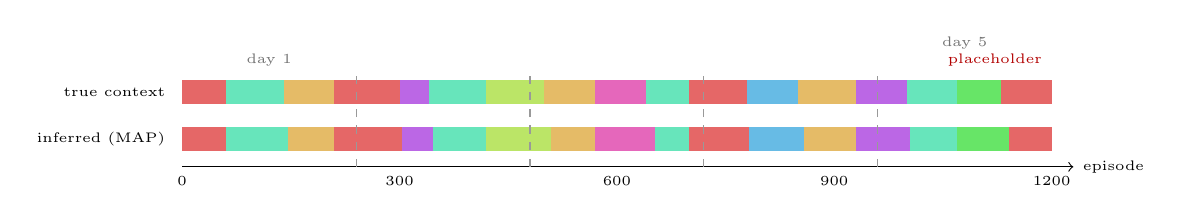
\begin{tikzpicture}[x=0.0092cm, y=1cm, font=\tiny]
% placeholder schedule: (start, end, context index)
\def\sched{0/60/0,60/140/4,140/210/1,210/300/0,300/340/7,340/420/4,420/500/2,500/570/1,570/640/8,640/700/4,700/780/0,780/850/5,850/930/1,930/1000/7,1000/1070/4,1070/1130/3,1130/1200/0}
\def\infer{0/60/0,60/146/4,146/210/1,210/303/0,303/346/7,346/420/4,420/509/2,509/570/1,570/652/8,652/700/4,700/783/0,783/858/5,858/930/1,930/1004/7,1004/1070/4,1070/1141/3,1141/1200/0}
\node[anchor=east] at (-10,1.2) {true context};
\node[anchor=east] at (-10,0.6) {inferred (MAP)};
\foreach \a/\b/\c in \sched {
  \pgfmathsetmacro{\hue}{\c/9}
  \definecolor{tmp}{hsb}{\hue,0.55,0.9}
  \fill[tmp] (\a,1.05) rectangle (\b,1.35);
}
\foreach \a/\b/\c in \infer {
  \pgfmathsetmacro{\hue}{\c/9}
  \definecolor{tmp}{hsb}{\hue,0.55,0.9}
  \fill[tmp] (\a,0.45) rectangle (\b,0.75);
}
\draw[->] (0,0.25) -- (1230,0.25) node[right] {episode};
\foreach \x in {0,300,600,900,1200} \node[below] at (\x,0.25) {\x};
\foreach \x in {240,480,720,960} \draw[black!40, dashed] (\x,0.25) -- (\x,1.45);
\node[text=black!55, anchor=south] at (120,1.4) {day 1};
\node[text=black!55, anchor=south] at (1080,1.62) {day 5};
\node[anchor=south east, text=red!70!black] at (1200,1.4) {placeholder};
\end{tikzpicture}
\caption{True and inferred contexts over the hardware deployment (placeholder schedule). Colours index the nine surface--load conditions; dashed lines mark day boundaries. Inferred switches lag true switches by the recognition time after contact, except where the cue alone identified the new condition.}
\label{fig:deployment}
\end{figure}
